% AI-assisted overview and figure integration, 25 October 2026.
% Methodology coordinator: Ayushi Negi. Review with the assigned section reviewers.
\section{Methodology}
\label{sec:Methodology}

The final implementation is available in the group's \href{https://github.com/AyushiNegi20/COSC2669-WIL-PROJECT}{WIL project repository}. FinTrace uses separate processes for preparing documents, retrieving evidence and producing answers. Figure~\ref{fig:fintrace_architecture} shows how structured financial tables and prose from the full reports reach the appropriate answer process. Both retain references to their sources. Evaluation questions and expected answers are kept outside the evidence used by the application.

\begin{figure}[!htbp]
\centering
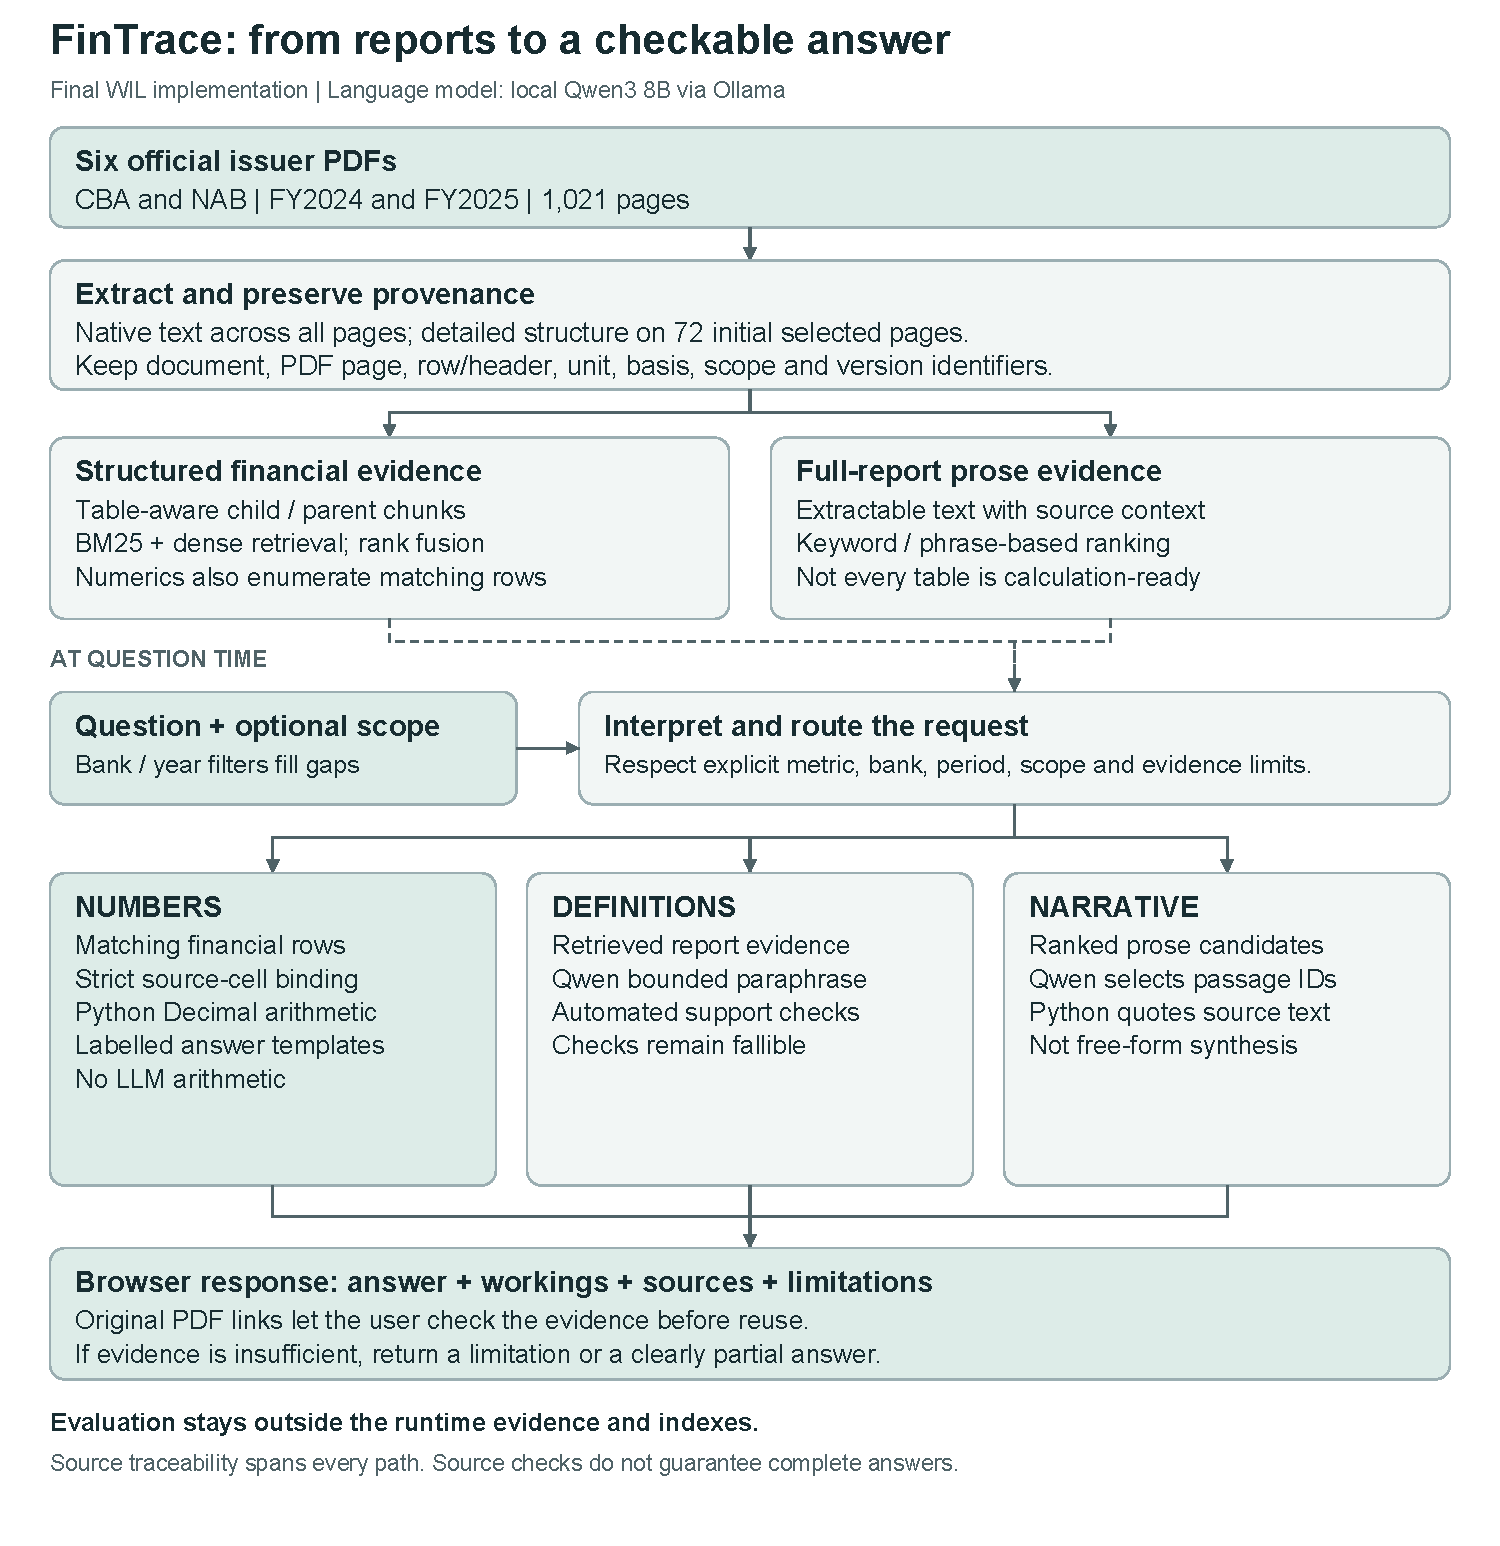
\includegraphics[width=0.98\linewidth,height=0.78\textheight,keepaspectratio]{fintrace_architecture.pdf}
\caption[FinTrace architecture]{Architecture of the final FinTrace implementation. Technical version details are recorded in Appendix~\ref{app:implementation_versions}. Structured evidence combines keyword and semantic retrieval, while prose uses keyword search followed by local model passage selection. Supported numerical answers link values to source cells and use Python for arithmetic. Qwen3 8B through Ollama supports passage selection and definitions. Dashed connections show evidence supplied to the relevant answer process~\cite{fintraceRuntime2026}.}
\label{fig:fintrace_architecture}
\end{figure}

% AI-assisted shared draft prepared at Ayushi's request on 25 October 2026.
% Assigned reviewer: Yash Keswani. Verify sources before approval; this is not personal authorship evidence.
\subsection{Data Sources and Scope}
\label{subsec:data_sources}

The knowledge base contains six official issuer reports for Commonwealth Bank of Australia (CBA) and National Australia Bank (NAB), covering FY2024 and FY2025. These comprise two CBA Profit Announcements, two NAB full-year results releases and two NAB Annual Reports, totalling 1,021 PDF pages. The source manifest records each document's title, issuer URL, reporting period and checksum~\cite{fintraceSources2026}. Results releases concentrate performance tables and management commentary~\cite{fintraceCBA2025,nabResults2025}; the NAB annual reports provide supporting accounting notes and reconciliations~\cite{nabAnnual2025}.

Banking provided a manageable domain with repeated measures and public evidence against which answers could be checked. Two years allow historical comparisons within a bank. However, CBA's year ends on 30 June and NAB's on 30 September: an identical financial-year label does not establish identical reporting periods. The prototype declines explicit cross-bank comparisons rather than treating them as directly comparable.

All reports received native-text extraction. An initial selection of 72 pages supported detailed structured extraction and checking; later indexing expanded searchable prose across the full reports. These are different coverage levels. Searchable text does not make every chart or table reliable enough for calculations. The original thirteen measure families defined a starting numerical scope, not a claim that other financial information was absent.

% Report section owner: Ayushi Negi
% AI-assisted working draft: verify against the cited extraction records before submission.
\subsection{PDF Extraction and Evidence Preservation}
\label{subsec:pdf_extraction}

We needed to extract more than the numbers on a page. A figure is only useful if it stays connected to its row label, year, unit and reporting basis. Each PDF is recorded with its issuer URL, document ID and SHA-256 checksum, a fingerprint that helps detect a changed file. This makes it possible to trace an answer back to the exact source used.

The extraction has two layers. pypdf first reads the text already stored in all 1,021 pages of the six PDFs. Docling then identifies table structure on an initial selection of 72 financial pages covering results, reconciliations, balances and supporting notes~\cite{doclingSoftware}. These pages contain selectable text, so optical character recognition (OCR) is disabled. Docling runs locally on CPU with four threads. Completed conversions are reused only when the source, pipeline and library versions match. Selecting 72 pages kept the more expensive table processing manageable; that number was a project boundary, not a technical requirement \cite{fintraceExtraction2026}.

We compared four libraries in six configurations on an 18-page development sample. The checks asked whether values followed the correct row in the correct order, not simply whether a number appeared somewhere on the page. Docling's results on this sample and its table representation supported its selection. The comparison was not a universal library ranking: the lighter table strategies were untuned and the sample also informed development. No separate, sealed extraction holdout was scored \cite{fintraceExtraction2026}.

Raw converter output is kept separately from cleaned evidence. The records retain cells, merged-cell spans, headings, page references, source coordinates and correction logs. In some CBA tables, invisible trailing brackets appeared in extracted text. A targeted pdfplumber check inspects the source characters and their colours before removing a bracket. Visible brackets denoting negative values are preserved. Cases that cannot be resolved stay flagged.

An additional audit scans every stored table cell. Simple numerical values are checked against the page text and the characters at their recorded coordinates. Mixed text and unresolved cases remain in a review queue. Agreement helps detect extraction inconsistencies, but does not establish that a number has been assigned the correct year, unit, basis or header \cite{fintraceExtractionFreeze2026}.

Full-report prose indexing later broadened searchable text, while calculations still required checked financial values. Extraction alone does not approve a figure for arithmetic. Chart-only content and unvalidated tables remain limitations. The next stage receives the extracted evidence and source records, not the evaluation answer keys.

% AI-assisted shared draft prepared at Ayushi's request on 25 October 2026.
% Assigned reviewer: Shriram Varadarajan. Confirm active implementation and citations.
\subsection{Chunking, Indexing and Retrieval}
\label{subsec:chunking_retrieval}

A useful financial chunk needs more than a nearby number. Splitting a table between its row label and year column can retain the digits while changing what an answer appears to mean. FinTrace therefore uses document structure as the starting point for checked financial evidence rather than cutting every fixed number of words~\cite{fintraceRetrieval2026}.

The chunk builder preserves headings, text blocks and table relationships. Table-row evidence carries relevant column headers and source context. Prose follows text boundaries, with oversized blocks split at sentence or word boundaries. Smaller child chunks support precise matching; parent records retain broader context and dependencies. Configured ceilings are 2,400 UTF-8 bytes per child and 10,000 per parent, with at most three table rows in a child. These are byte limits, not token counts. Nearby footnotes can be context, but proximity alone does not establish which figure they qualify. Ambiguous table evidence is quarantined rather than promoted into calculation-ready material.

Each unit retains identifiers for its bank, report, reporting year, PDF page, source blocks or rows and parent. Units, basis, scope and report vintage are carried where resolved. These fields support filtering and let citations identify a PDF page even when printed numbering differs. Context enrichment makes a short row searchable without inventing missing headers.

Two search paths are maintained. Structured evidence combines BM25 keyword retrieval with dense retrieval using Qwen3-Embedding-0.6B~\cite{qwenEmbedding}. BM25 rewards informative shared terms; dense representations can match related wording. Reciprocal rank fusion combines their rankings. Dense vectors are local NumPy arrays searched by exact similarity, not a hosted database. Tokenizer checks constrain embedding inputs, and answer evidence has a separate packing budget. Appendix~\ref{app:runtime_details} records the settings; an entire report is not supplied to the model.

Full-report prose instead uses lexical ranking with contextual and phrase signals, followed by local-model passage selection. It is not a dense index of all 1,021 pages. This broadens access to explanations without validating every table for numerical use.

Numerical lookup considers indexed financial rows matching the bank and measure rather than relying only on hybrid top-five results. Strict binding then checks row identity, native digits, period, unit, basis, scope, vintage and conflicts. Housing lending must not become total loans, and net interest income must not become net interest margin. Explicit question constraints take precedence over optional interface filters~\cite{fintraceRuntime2026}.

Fixed-size splitting and additional reranking were considered, but choices were guided by observed failures rather than assumed sophistication. Historical development checks informed chunk and query handling; they are not blind estimates of current accuracy. Retrieval relevance, correct cell binding and answer completeness remain separate outcomes. A correct citation can identify useful evidence while leaving a multi-part question only partly answered. Missing retrieved evidence likewise does not establish that information is absent from the PDF.

% AI-assisted shared draft prepared at Ayushi's request on 25 October 2026.
% Assigned reviewer: Yash Keswani. Verify configuration and account for AI assistance.
\subsection{Answer production and model configuration}
\label{subsec:answer_production}

FinTrace handles numerical requests, definitions and narrative questions separately because each requires different checks~\cite{fintraceRuntime2026}. Numerical requests are matched to extracted source cells while retaining the company, year, unit, financial basis, business scope and report version. Python displays checked values through templates and uses decimal arithmetic for supported comparisons. Absolute change is the later value minus the earlier value; relative change divides this difference by the earlier value. Changes in percentage measures are reported in percentage points, with basis points where supported. The language model does not calculate financial results. General profit questions return available labelled alternatives rather than requiring users to choose a financial definition first.

Definitions use report evidence with controlled paraphrasing by the local model and automated support checks. Narrative questions use keyword retrieval followed by Qwen passage selection. The application then displays quotations from the selected passages. The active \texttt{source\_selection} setting therefore differs from unrestricted answer generation. Checks of identifiers and quotations prevent invented excerpts, but do not independently establish whether the selected evidence fully answers the question. For mixed requests, an incomplete explanation remains visible even if the numerical part succeeds.

The local model is \texttt{qwen3:8b} through Ollama, using the Q4\_K\_M quantised distribution with reduced precision weights~\cite{qwenOllama}. It was not trained or fine-tuned for this project. The configured context is 16,384 tokens. Output limits and sampling settings are recorded in Appendix~\ref{app:runtime_details}. A 35-second timeout applies to each call rather than to a whole question, and evidence size is limited separately~\cite{fintraceRuntime2026}.

Experiments with local models and a small comparison using Groq informed model selection. These development examples do not establish general superiority over other models. Testing also showed that fluent generation could repeat an incorrectly selected financial measure. Generation was therefore removed from the numerical process while source checks were retained. Local inference avoids provider charges per token but uses laptop resources and can be slower when models first load. When evidence is insufficient, the response describes the limitation rather than claiming the full report lacks an answer. Automated model review is treated as a safeguard rather than independent verification.

% AI-assisted shared draft prepared at Ayushi's request on 25 October 2026.
% Assigned reviewer: Guruprasad Simimath. Live screenshots captured for the report on 25 October 2026.
\subsection{Frontend and user workflow}
\label{subsec:frontend_workflow}

The frontend is a custom HTML, CSS and JavaScript application connected to the RAG pipeline through a local Python HTTP server. It displays answers, calculations, source references and evidence limitations. Health checks support the connection indicator, while the document library endpoint provides the report list~\cite{fintraceRuntime2026}.

Users can ask a question directly or select optional bank and financial year filters. A bank or year named in the question takes precedence; filters supply missing context. Users do not need to classify their request as a lookup, definition or explanation. The interface accepts up to 2,000 characters and retains up to eight successful responses in the current browser tab. This history is not a persistent account or an archive available on other devices.

Financial labels remain visible beside figures. Supported comparisons show their calculation workings, and numbered references lead to extracted evidence and the original PDF page. Responses can be copied or downloaded as JSON, a structured format for inspecting the result. These controls let an analyst examine how an answer was produced rather than relying on its wording alone.

Partial answers and evidence limitations are displayed explicitly. A quotation selected from a report is distinguished from a generated explanation because a relevant passage may not establish a requested ranking or cause. Figures~\ref{fig:frontend_profit} and~\ref{fig:frontend_comparison} illustrate two live examples already used during development. They demonstrate the interface rather than provide a new accuracy or latency assessment.

\begin{figure}[!htbp]
\centering
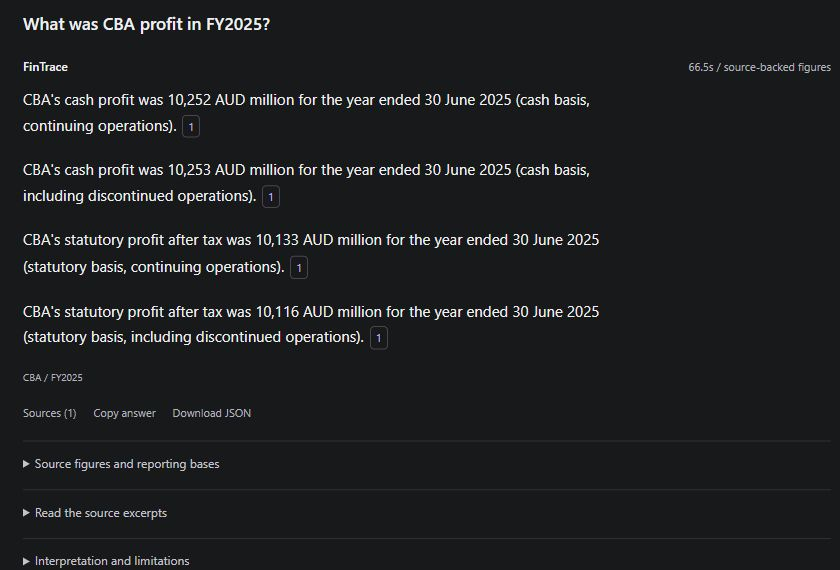
\includegraphics[width=0.98\linewidth]{frontend_profit.png}
\caption[Frontend: labelled profit alternatives]{Live interface response to ``What was CBA profit in FY2025?'' Four figures linked to source cells distinguish cash/statutory basis and continuing/total operations. The numbered references identify CBA's FY2025 Profit Announcement, PDF page 18~\cite{fintraceCBA2025}.}
\label{fig:frontend_profit}
\end{figure}

\begin{figure}[!htbp]
\centering
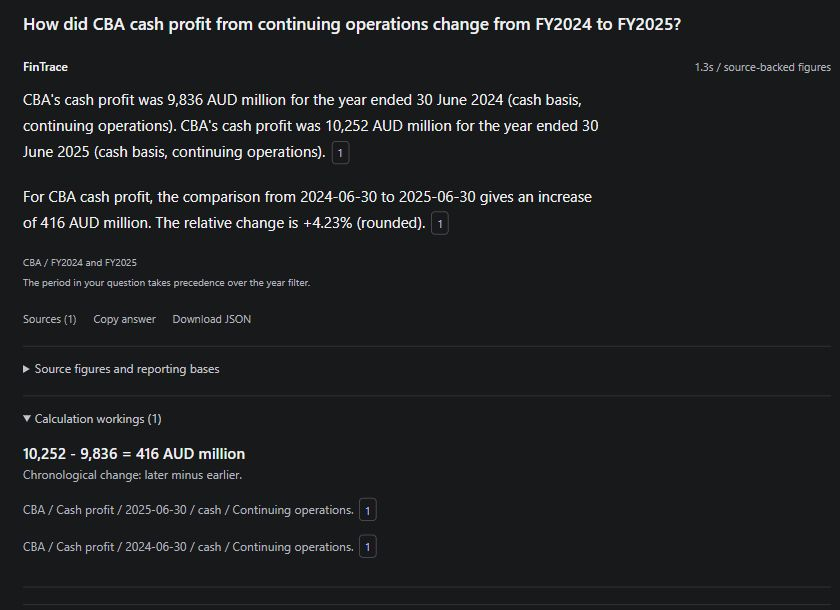
\includegraphics[width=0.98\linewidth]{frontend_comparison.png}
\caption[Frontend: comparison and calculation workings]{Live interface comparison of CBA continuing cash profit from FY2024 to FY2025. The expanded workings show AUD~10,252 million minus AUD~9,836 million, giving AUD~416 million; the answer reports approximately 4.23\% relative growth. Operand references lead to PDF page 18 of the FY2025 report. Screenshots are illustrative runs, not timing guarantees.}
\label{fig:frontend_comparison}
\end{figure}

The prototype runs locally for a single user. Its evidence, models and indexes require installation beyond cloning the repository. Model startup and competition for GPU resources can affect response time. Checks of interface state and server behaviour were recorded separately from financial answer assessment. Formal accessibility, multi-user load and analyst usability studies remain future work.

% AI-assisted shared draft prepared at Ayushi's request on 25 October 2026.
% Assigned reviewer: Janhavi Maheshwar Ghate. Verify packets and scoring with Hashini.
\subsection{Evaluation design and scoring criteria}
\label{subsec:evaluation_design}

Evaluation distinguished finding relevant evidence from producing a correct and complete answer. A response may contain a valid number yet use the wrong financial basis, omit a requested part or cite an unrelated page. We therefore assessed retrieval, financial correctness, completeness, citation support, appropriate refusals and response time separately~\cite{fintraceEval2026}.

Questions covered lookups, comparisons across years within a bank, calculations, definitions, management explanations and ambiguous wording. Boundary cases tested unavailable years, future outcomes, other companies, live prices and personal investment advice. Reference answers record the document, page, reporting period, unit, financial basis and business scope. Assessment also considers whether the requested information is available within the prototype's searchable or checked evidence.

Responses to answerable questions are classified as complete, partial, incorrect or unnecessarily declined. An appropriate refusal concerns unavailable information or a clearly stated scope boundary. Declining an answerable request remains a coverage or effectiveness limitation even when it avoids fabrication. Runtime errors are recorded separately. Correctness requires the right financial context; completeness requires every requested part, including both comparison values and the calculation when a change is requested.

Hit@5 measures whether relevant evidence appears among the first five retrieval results. Mean reciprocal rank rewards placing relevant evidence earlier. nDCG@5 evaluates the order of the first five results relative to relevance judgments. These retrieval measures require saved rankings and relevance labels; they cannot be inferred from final citations. Numerical matching can also consider rows outside the first five results. Citation checks instead establish whether the cited page supports a claim. Arithmetic checks inspect operands, formula, units and rounding, distinguishing percentage points from relative percentage growth.

Development tests guided fixes, while regression tests checked previously observed behaviour. Separate AI-assisted assessments used questions held outside the runtime repository, not an external human panel. Because the archived question file names both issuer PDFs and the development metric catalogue as references, separate authorship does not establish an entirely unseen assessment based only on the reports. Once questions informed a fix, they became development evidence. Software test counts and successful HTTP responses are not financial answer accuracy. Each result is therefore reported with its software version and sample size, separating appropriate refusals from missed answerable questions.

% AI-assisted shared draft prepared at Ayushi's request on 25 October 2026.
% Assigned reviewer: Hashini Santhanakrishnan. Confirm original runs with Janhavi.
\subsection{Evaluation procedure and validity safeguards}
\label{subsec:evaluation_procedure}

Before assessment, the procedure records the software version, model configuration and evidence files. Integrity checks compare the application and source files against a recorded list of checksums before and after testing. This establishes whether the system changed during the assessment, rather than whether its answers are financially correct~\cite{fintraceEval2026}.

Questions and expected answers remain separate from the runtime evidence. The evaluation script uses \texttt{serve\_fintrace\_demo.build\_backend()} so that it tests the configured application rather than generic defaults. Every first response is preserved, including errors and fallbacks, without retrying until a favourable answer appears. Response time is recorded separately from correctness.

Assessment examines the complete response, including displayed text, structured claims, calculations, quotations and limitations. This avoids an earlier evaluation adapter error that overlooked calculations stored outside the prose. Claims are checked against cited pages for the correct row, year, unit, financial basis, business scope and report version. Equivalent units and reasonable rounding are acceptable; substituting a neighbouring financial measure is not. An explanation that gives a correct figure without the requested reasons is incomplete.

Disagreements are investigated against the source before changing an answer or reference key. Original expectations and failed responses are retained alongside corrections. When an earlier year's figure comes from a later report's comparative column, that publication is identified. A difference from the original report does not by itself establish a formal restatement. Comparisons use compatible columns when calculating changes~\cite{fintraceCandidate2026}.

The main validity limits are small, deliberately selected question sets, AI-assisted judgments and changes in coverage during development. No independent human panel or controlled analyst study was conducted. Questions used for tuning cannot establish performance on unseen requests. Responses and timing may also vary between runs. Earlier results therefore apply to the versions tested, while the frontend screenshots illustrate functionality rather than provide a fresh accuracy estimate.

